\documentclass[12pt, titlepage]{article}

\usepackage{graphicx}
\usepackage{float}
\usepackage{booktabs}
\usepackage{tabularx}
\usepackage{hyperref}
\hypersetup{
    colorlinks,
    citecolor=black,
    filecolor=black,
    linkcolor=red,
    urlcolor=blue
}
\usepackage[round]{natbib}

%% Comments

\usepackage{color}

\newif\ifcomments\commentstrue %displays comments
%\newif\ifcomments\commentsfalse %so that comments do not display

\ifcomments
\newcommand{\authornote}[3]{\textcolor{#1}{[#3 ---#2]}}
\newcommand{\todo}[1]{\textcolor{red}{[TODO: #1]}}
\else
\newcommand{\authornote}[3]{}
\newcommand{\todo}[1]{}
\fi

\newcommand{\wss}[1]{\authornote{blue}{SS}{#1}} 
\newcommand{\plt}[1]{\authornote{magenta}{TPLT}{#1}} %For explanation of the template
\newcommand{\an}[1]{\authornote{cyan}{Author}{#1}}

%% Common Parts

\newcommand{\progname}{Software Engineering} % PUT YOUR PROGRAM NAME HERE
\newcommand{\authname}{Team \#11, OKKM Insights
\\ Mathew Petronilho
\\ Oleg Glotov
\\ Kyle McMaster
\\ Kartik Chaudhari} % AUTHOR NAMES                  

\usepackage{hyperref}
    \hypersetup{colorlinks=true, linkcolor=blue, citecolor=blue, filecolor=blue,
                urlcolor=blue, unicode=false}
    \urlstyle{same}
                                


\begin{document}

\title{Verification and Validation Report: \progname} 
\author{\authname}
\date{\today}
	
\maketitle

\pagenumbering{roman}

\section{Revision History}

\begin{tabularx}{\textwidth}{p{3cm}p{2cm}X}
\toprule {\bf Date} & {\bf Version} & {\bf Notes}\\
\midrule
Date 1 & 1.0 & Notes\\
Date 2 & 1.1 & Notes\\
\bottomrule
\end{tabularx}

~\newpage

\section{Symbols, Abbreviations and Acronyms}

\renewcommand{\arraystretch}{1.2}
\begin{tabular}{l l} 
  \toprule		
  \textbf{symbol} & \textbf{description}\\
  \midrule 
  T & Test\\
  \bottomrule
\end{tabular}\\

\wss{symbols, abbreviations or acronyms -- you can reference the SRS tables if needed}

\newpage

\tableofcontents

\listoftables %if appropriate

\listoffigures %if appropriate

\newpage

\pagenumbering{arabic}

This document ...

\section{Functional Requirements Evaluation}

\section{Nonfunctional Requirements Evaluation}

\subsection{Usability}
		
\subsection{Performance}

\subsection{etc.}
	
\section{Comparison to Existing Implementation}	

This section will not be appropriate for every project.

\section{Unit Testing}
\subsection{Front-end}
Please refer to the tests folder in the frontend directory found \href{https://github.com/OKKM-insights/frontend/tree/main/tests/__tests__}{here}.
\subsubsection{Rendering of a Component}
\begin{itemize}
    \item Description: A unit test was written for each component to ensure that it renders without error
    \item Inputs: The component
    \item Expected Outputs: The component renders 
    \item Result: Pass
\end{itemize}
\subsubsection{Open Pop Up}
\begin{itemize}
    \item Description: A unit test was written for each pop up component to ensure the pop up appears when open
    \item Inputs: open := true
    \item Expected Outputs: The pop up renders 
    \item Result: Pass
\end{itemize}
\subsubsection{Close Pop Up}
\begin{itemize}
    \item Description: A unit test was written for each pop up component to ensure the pop up does not appear when closed
    \item Inputs: open := false
    \item Expected Outputs: The pop up does not render 
    \item Result: Pass
\end{itemize}
\subsubsection{Header Logged In}
\begin{itemize}
    \item Description: Ensure the header renders the right things when the user is logged in
    \item Inputs: logged in := true
    \item Expected Outputs: The header should contain the log out button and profile button
    \item Result: Pass
\end{itemize}
\subsubsection{Header Logged Out}
\begin{itemize}
    \item Description: Ensure the header renders the right things when the user is logged out
    \item Inputs: logged in := false
    \item Expected Outputs: The header should contain the log in button and register button
    \item Result: Pass
\end{itemize}
\subsubsection{Header Re-directions}
\begin{itemize}
    \item Description: Ensure the headers buttons redirect to the expected link
    \item Inputs: N/A
    \item Expected Outputs: The header redirects to the login on pressing the login button, register on pressing the register button, home when clicking the logout button, and edit profile information when clicking the profile button 
    \item Result: Pass
\end{itemize}
\subsubsection{Login Success}
\begin{itemize}
    \item Description: Ensure the authorization context is set up upon successful login
    \item Inputs: valid email and password
    \item Expected Outputs: Login is successful and authorization context is set up
    \item Result: Pass
\end{itemize}
\subsubsection{Login Fail}
\begin{itemize}
    \item Description: Ensure error message is displayed on login fail
    \item Inputs: invalid email and password
    \item Expected Outputs: Message saying invalid credentials
    \item Result: Pass
\end{itemize}
\subsubsection{New Project Validation}
\begin{itemize}
    \item Description: Ensure required inputs are filled and notify the user if not
    \item Inputs: empty required fields such as name
    \item Expected Outputs: Message saying what required fields have not been filled in
    \item Result: Pass
\end{itemize}
\subsubsection{New Project Creation Success}
\begin{itemize}
    \item Description: Ensure form submission occurs and success pop up is activated when server creates project
    \item Inputs: Entirely filled out project creation form
    \item Expected Outputs: Success pop up shown
    \item Result: Pass
\end{itemize}
\subsubsection{New Project Creation Failure}
\begin{itemize}
    \item Description: Ensure form submission occurs and failure pop up is activated when a server side error occurs
    \item Inputs: Entirely filled out project creation form
    \item Expected Outputs: Failure pop up shown
    \item Result: Pass
\end{itemize}
\subsubsection{Project Section renders all projects}
\begin{itemize}
    \item Description: Ensure projects section component renders all projects given to it
    \item Inputs: A list of projects
    \item Expected Outputs: Each project has its own project card on the page
    \item Result: Pass
\end{itemize}
\subsubsection{Project Tile Navigation}
\begin{itemize}
    \item Description: Ensure project tile redirects to the correct page
    \item Inputs: tile type
    \item Expected Outputs: When the tile type is label, it redirects to the label project. When the tile type is client, it redirects to project insights.
    \item Result: Pass
\end{itemize}
\subsubsection{Register Dynamic Password Validation}
\begin{itemize}
    \item Description: Ensure the password conditions show as satisfied when given a valid password
    \item Inputs: A valid password
    \item Expected Outputs: Password conditions show as satisfied
    \item Result: Pass
\end{itemize}
\subsubsection{Register Success}
\begin{itemize}
    \item Description: Ensure the form is submitted, shows a success pop up, and redirect
    \item Inputs: valid email and password
    \item Expected Outputs: Success pop up comes up and redirected to the login page
    \item Result: Pass
\end{itemize}
\subsubsection{Register Fail}
\begin{itemize}
    \item Description: Ensure the user is notified if the account already exists
    \item Inputs: duplicate email
    \item Expected Outputs: Message saying the account already exists
    \item Result: Pass
\end{itemize}
\subsubsection{Update Info Success}
\begin{itemize}
    \item Description: Ensure the form is submitted and the new information is now displayed
    \item Inputs: valid email change
    \item Expected Outputs: Email on the account information page is updated to the new email
    \item Result: Pass
\end{itemize}
\subsubsection{Update Info Fail}
\begin{itemize}
    \item Description: Ensure the user is notified if the account already exists, do not allow update
    \item Inputs: duplicate email
    \item Expected Outputs: Message saying the account already exists
    \item Result: Pass
\end{itemize}

\section{Changes Due to Testing}

\wss{This section should highlight how feedback from the users and from 
the supervisor (when one exists) shaped the final product.  In particular 
the feedback from the Rev 0 demo to the supervisor (or to potential users) 
should be highlighted.}

\subsection{Changes to Front-end}
Our labeling tool was largely refactored to incorporate the feedback we received from our usability testing. We also considered some of the unit testing outcomes. These changes included:
\begin{itemize}
    \item Added clearer visual feedback to all the buttons present in the labeling tool. Also made the currently selected label type more obvious to the user.
    \item Changed the contextual pop ups to include more detailed descriptions and any short cuts associated with a button.
    \item Added more details and made steps more granular in the help walk-through of the labeling tool. These additional details should help the user in further understanding what they need to do.
    \item Changed the text of the main submission buttons so that it was clear what would happen when they were pressed. For example, submit was renamed to "submit labels".
    \item Fixed a bug where the tool would get stuck if the submit button was pushed when there was no labels made.
    \item The label button now stays selected after a label is created so the user can seamlessly label multiple objects of the same class without having to reselect it every time.
    \item A visual gif will be added to show the basic process of creating a label so that it is clear the labels are to be drawn on the image.
    \item Rather than have tools spread out, they have all been condensed into an easy access toolbar.
    \item New button was added to reset zoom, contrast, brightness and image position back to its initial state.
    \item Removed white space.
    \item Removed help button when the project was complete.
\end{itemize}

\section{Automated Testing}
Automated testing and linting have been implemented in the frontend and backend repositories, as described in section 7.2 of the \href{https://github.com/OKKM-insights/OKKM.insights/blob/main/docs/DevelopmentPlan/DevelopmentPlan.pdf}{Development Plan}.

		
\section{Trace to Requirements}
The traceability from tests to requirements can be seen in section 4.3 of the \href{https://github.com/OKKM-insights/OKKM.insights/blob/main/docs/VnVPlan/VnVPlan.pdf}{VnV Plan}.
		
\section{Trace to Modules}
The traceability from requirements to modules can be seen in section 8 of the \href{https://github.com/OKKM-insights/OKKM.insights/blob/main/docs/Design/SoftArchitecture/MG.pdf}{Module Guide}. The tests that cover a specific requirement also cover the modules associated with that requirement.	

\section{Code Coverage Metrics}
\subsection{Front-end Coverage}
The coverage results of the front-end unit testing can be seen in Figure~\ref{fig:FE_coverage}. Perfect coverage was not achieved, but we believe our unit tests supplemented with our manual and usability tests provide sufficient coverage of the code.
\begin{figure}[H]
    \centering
    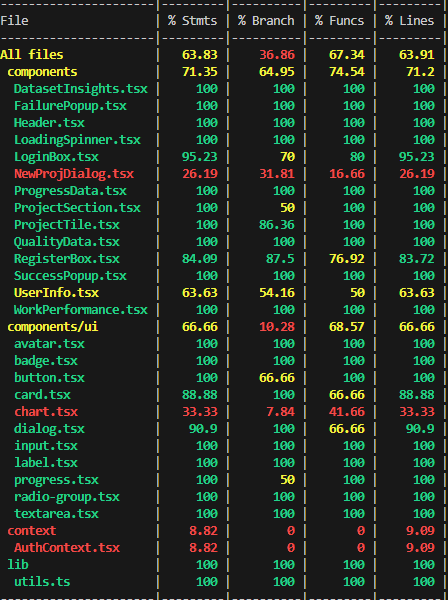
\includegraphics[width=0.5\linewidth]{FE_coverage.png}
    \caption{Front-end Unit Testing Coverage Results}
    \label{fig:FE_coverage}
\end{figure}

\bibliographystyle{plainnat}
\bibliography{../../refs/References}

\newpage{}
\section*{Appendix --- Reflection}

The information in this section will be used to evaluate the team members on the
graduate attribute of Reflection.

The purpose of reflection questions is to give you a chance to assess your own
learning and that of your group as a whole, and to find ways to improve in the
future. Reflection is an important part of the learning process.  Reflection is
also an essential component of a successful software development process.  

Reflections are most interesting and useful when they're honest, even if the
stories they tell are imperfect. You will be marked based on your depth of
thought and analysis, and not based on the content of the reflections
themselves. Thus, for full marks we encourage you to answer openly and honestly
and to avoid simply writing ``what you think the evaluator wants to hear.''

Please answer the following questions.  Some questions can be answered on the
team level, but where appropriate, each team member should write their own
response:


\begin{enumerate}
  \item What went well while writing this deliverable? 
  \item What pain points did you experience during this deliverable, and how
    did you resolve them?
  \item Which parts of this document stemmed from speaking to your client(s) or
  a proxy (e.g. your peers)? Which ones were not, and why?
  \item In what ways was the Verification and Validation (VnV) Plan different
  from the activities that were actually conducted for VnV?  If there were
  differences, what changes required the modification in the plan?  Why did
  these changes occur?  Would you be able to anticipate these changes in future
  projects?  If there weren't any differences, how was your team able to clearly
  predict a feasible amount of effort and the right tasks needed to build the
  evidence that demonstrates the required quality?  (It is expected that most
  teams will have had to deviate from their original VnV Plan.)
\end{enumerate}

\end{document}